\documentclass{article}
\usepackage{amsmath, amssymb, mdwlist, graphicx, hyperref}
\usepackage{listings,color}
\usepackage{enumitem}
\usepackage{wrapfig}
\usepackage[usenames,dvipsnames]{xcolor}
\definecolor{gray}{rgb}{0.97,0.97,0.97}
\lstset{%
language=C,%
%backgroundcolor=\color{gray},
emph={putpixel},
emphstyle=\bf,
tabsize=4,
framesep=5pt,
mathescape=true,
xleftmargin=0.1cm,
xrightmargin=0.1cm,
frame=lines,
%basicstyle=\ttfamily,
%keywordstyle=\color{Blue},
%commentstyle=\color{OliveGreen},
%stringstyle=\color{MidnightBlue},
columns=flexible,
%showstringspaces=false
}

\newcommand{\mpar}[1]{\marginpar{\textit{#1}}}
\newcommand{\norm}[1]{\Vert #1 \Vert}
\DeclareMathOperator{\argmax}{argmax}
\DeclareMathOperator{\argmin}{argmin}
\newenvironment{solution}{\paragraph{Solution.}$\,$ }{\vskip 3mm\hrule}
\newenvironment{exercise}[2]{\paragraph{Exercise #1 (#2pt).} }{
\medskip}
\newcommand{\bbR}{\mathbb{R}}
\newcommand{\bw}{\mathbf{w}}
\newcommand{\bx}{\mathbf{x}}
\newcommand{\bd}{\mathbf{d}}
\newcommand{\bb}{\mathbf{b}}
\newcommand{\by}{\mathbf{y}}
\newcommand{\bzero}{\mathbf{0}}
\newcommand{\bz}{\mathbf{z}}
\newcommand{\bSigma}{\mathbf{\Sigma}}
\newcommand{\bp}{\mathbf{p}}
\newcommand{\bP}{\mathbf{P}}
\newcommand{\bm}{\mathbf{m}}
\newcommand{\bc}{\mathbf{c}}
\newcommand{\bM}{\mathbf{M}}
\newcommand{\bV}{\mathbf{V}}
\newcommand{\bK}{\mathbf{K}}
\newcommand{\bD}{\mathbf{D}}
\newcommand{\bA}{\mathbf{A}}
\newcommand{\bX}{\mathbf{X}}
\newcommand{\bY}{\mathbf{Y}}
\newcommand{\bR}{\mathbf{R}}
\newcommand{\bI}{\mathbf{I}}
\newcommand{\bS}{\mathbf{S}}
\newcommand{\bT}{\mathbf{T}}
\newcommand{\balpha}{\boldsymbol{\alpha}}
\newcommand{\pt}[2]{\left(\begin{array}{c}#1\\#2\end{array}\right)}

\begin{document}
\title{MTAT.03.015 Computer Graphics (Fall 2013)\\
Exercise session XIV: OGRE}
\author{Ilya Kuzovkin, Konstantin Tretyakov}
\date{December 9, 2013}
\maketitle

In this exercise session we will have a look at the high-level graphics engine OGRE\footnote{\url{http://www.ogre3d.org/}}. We will see how the concepts we know about are included into the OGRE engine, making our life easier. Lighting, materials, shadows, environment mapping and other techniques are accessible by adding few lines of code, without the need to implement the annoying details on our own.

As before, the solutions will have to be submitted as a zipped project directory. Please, keep Windows libraries and project files in the archive, even if you work on Linux or Mac.

You can always seek for additional information and help in the OGRE tutorials \footnote{\url{http://www.ogre3d.org/tikiwiki/tiki-index.php?page=Tutorials}} and reference pages\footnote{\url{http://www.ogre3d.org/docs/api/html/}}.

Before proceeding, check out the \texttt{README.txt} file in the practice files archive for some important notes. In particular, if you work on Linux, you will need to install OGRE before proceeding (for Windows, all the necessary libraries are provided). In Debian-based systems this can be done using a command like the following:
\begin{verbatim}
    $ sudo apt-get install libogre-1.8-dev libois-dev
\end{verbatim}

\section{Structure of the application}
We start by comparing the structure of the application to the familiar structure we have been using so far. Open the project \verb#1_OgreTriangle# and read through the code in the \verb#triangle.cpp# file. Compare it to GLUT-based applications we have seen before.

\begin{exercise}{1}{0.5}
Add a small square which will fly around the triangle and rotate around its own center. For that you will need to:
\begin{enumerate}
	\item Create a new \verb#Ogre::ManualObject# object using \verb#createManualObject()# method of the scene manager.
	\item Describe the vertices of your square. Note that, in contrast to OpenGL, in OGRE we \emph{first} write the \texttt{position} command to create the vertex itself, and then describe its attributes, such as color. The order in which the vertices are specified will depend on which type of \verb#Ogre::RenderOperation#\footnote{\url{http://www.ogre3d.org/docs/api/html/classOgre_1_1RenderOperation.html}} (triangle list, triangle strip or triangle fan) you decide to use. 
	\item Create an \verb#Ogre::SceneNode#, and attach the new object to it.
	\item Use this \verb#SceneNode# to animate the object (update its position) in the \verb#frameRenderingQueued()# method (which is an analog of the \verb#idleFunc()# we were using in GLUT).
\end{enumerate}
The existing code for creating the triangle will serve you as an example. The result should look something like this:
\begin{center}
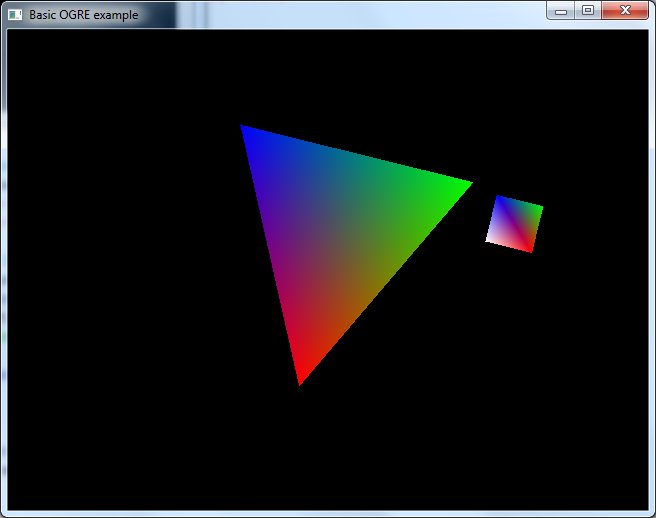
\includegraphics[width=0.7\textwidth]{ex1.png}
\end{center}
\end{exercise}

\section{Lighting, materials and textures}

Open the project \verb#2_OgreLighting#. The general structure is the same as before. Study the code in \verb#createLitSphereScene()#. Here we configure our scene: create a sphere, add material specification to it, enable lighting and shadows.

In Exercise Session 9, which was about different types of shadows, we implemented three different shadow techniques. You might remember that for implementing \emph{stencil shadows}, for example, you first needed to create shadow volume objects and after that implement the logic by carefully playing with stencil, color and depth buffers. OGRE allows you to enable shadows with literally one line of code\footnote{See more \url{http://www.ogre3d.org/tikiwiki/tiki-index.php?page=Basic+Tutorial+2}}. This line is already written for you in the \texttt{createLitSphereScene()} function, but is commented. Find and uncomment it.

Now pay attention to these lines in the middle of the \verb#run()# function:
\begin{verbatim}
 Ogre::ResourceGroupManager::getSingleton().
                     addResourceLocation("../data", "FileSystem");
 Ogre::ResourceGroupManager::getSingleton().
                     initialiseAllResourceGroups();
\end{verbatim}
In reality graphics-heavy applications would often use many external \emph{resource files}, to specify meshes, textures, materials, and other things. The first line tells OGRE where to look for the resources: data files (textures, meshes, etc.) and scripts. The second line instructs it to read in resource descriptions and initialise \emph{resource groups}.

Have a look at the \verb#Examples.material# file\footnote{This is a file from the OGRE SDK, used in many examples and tutorials.} in the \verb#data# folder and try to apply some of materials described there to our sphere. For example, try
\begin{verbatim}
    sphere->setMaterialName("Examples/WaterStream");
\end{verbatim} 
If you would like to try other example materials you should download the full OGRE SDK\footnote{\url{http://www.ogre3d.org/download/sdk}} and copy the resources (e.g. textures) needed for each particular example from the SDK to our \verb#data# folder.

\begin{exercise}{2}{1}
Create two new files \verb#data/Sphere.material# and \verb#data/# \verb#Plane.material#. Those will be used to describe materials of our objects.
\begin{enumerate}
	\item[1.] Use examples in \verb#data/Examples.material# and the relevant OGRE manual pages\footnote{\url{http://www.ogre3d.org/docs/manual/manual_16.html}} to create a material script for the sphere, which exactly reproduces material parameters we have specified in the code. The result should look exactly the same: red sphere with white specular spot on it.
\end{enumerate}
Next, let us see how texture mapping is done within \verb#.material# scripts.
\begin{enumerate}
	\item[2.] Find material examples in \verb#data/Examples.material#, which have a \\ \verb#texture_unit# section. Note that textures can also be animated (e.g. \verb#Examples/WaterStream#).
	\item[3.] Describe the material with a texture in the \verb#Plane.material# file. Pick some favourite picture of yours for the texture.
\end{enumerate}
Note that you can use \verb#WASD# keys and the mouse to control the camera in this project. This is enabled by the invocation of the \texttt{controlCamera} utility method of the \texttt{SimpleMouseAndKeyboardListener} class, provided in \verb#input_util.h#.

\end{exercise}

\begin{exercise}{3*}{0.5}
A realistic scene requires some background. A simple way to provide such background is by enabling a ``sky box'', which is simply a cube-mapped texture, applied to the background around the scene. To specify a cube-mapped texture you need 6 image files, which have common prefix \verb#mytexture_# and six suffixes, one for each side of the cube: \verb#bk#, \verb#dn#, \verb#fr#, \verb#lf#, \verb#rt#, \verb#up#. See the images \verb#stevecube_*.jpg# in our \verb#data# folder. Have a look at the tutorial\footnote{\url{http://www.ogre3d.org/tikiwiki/tiki-index.php?page=Basic+Tutorial+3}} and add a sky box to our scene. You can use the provided images or make up your own.
\end{exercise}

\begin{exercise}{4*}{0.5}
Look at the scene now. You might feel the urge to make the sphere reflective. The simplest way to do it would be to apply the cube map texture from the previous exercise as a \verb#cubic_reflection# type of environment map to the sphere material. This would not be completely correct, however, as the reflection would not take into account the ``floor'' nor any other objects that might appear in the scene. To make proper reflections the cube map must be generated \emph{dynamically} by actually rendering the scene from the point of view of the sphere. Study the code in \verb#examples/CubeMapping/include/# \verb#CubeMapping.h# and use it to add a dynamically changing cubic reflection map onto the sphere. Here is an approximate description of the steps you need to do to implement dynamical cube mapping:
\begin{enumerate}[noitemsep]
	\item Make our \verb#Application# class inherit \verb#Ogre::RenderTargetListener#
	\item Make use of \verb#preRenderTargetUpdate()# method
	\item Add some global variables
	\item Create cube map texture in the same way as it is done in \verb#createCubeMap()#
	\item Use \verb#Examples/DynamicCubeMap# to create a new material in our \\ \verb#Sphere.material# script
	\item Enable this material using \verb#setMaterialName()# method 	
\end{enumerate}
Note how we use an additional camera to update textures used for the cube. Since textures are updated on each frame you will get actual dynamic reflections.
\end{exercise}

\newpage
After completing exercises 2, 3 and 4 your scene might look something like this. 
\begin{center}
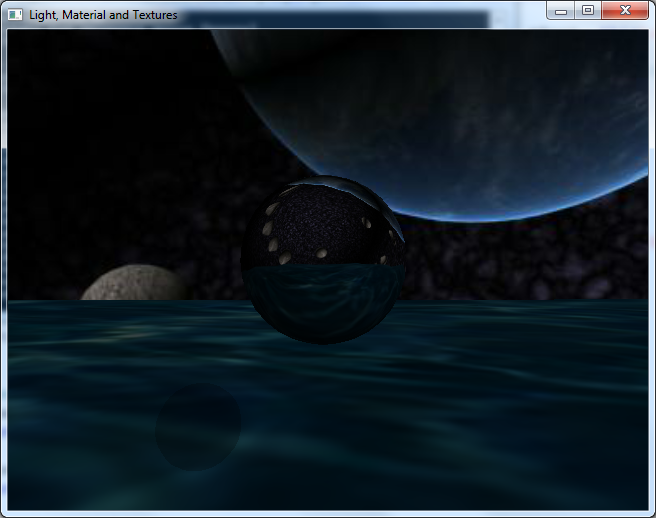
\includegraphics[width=0.7\textwidth]{textures.png}
\end{center}



\section{Meshes and character animation}

Now let us study how OGRE works with meshes. Open the project \verb#3_OgreMesh#. Meshes are handled as any other object we have seen before: they are entities, they are attached to a \verb#SceneNode# and you can specify materials, textures and shadows in the exactly same way as we have seen before. Most importantly, however, a complex mesh can be loaded from a resource file. Have a look at \verb#createOgreScene()# routine to see how mesh is loaded and attached to the scene.

\begin{exercise}{5}{0.5}
Let us try to animate the mesh using skeletal animation. In the \verb#data/Character# directory (which we use as resource location for this project) among other things we have a \verb#Sinbad.skeleton# file. It describes the armature (set of bones) for our character and 13 different keyframe animations for that armature\footnote{\url{http://www.ogre3d.org/docs/manual/manual_75.html}}. The animations are named \verb#IdleBase#, \verb#IdleTop#, \verb#RunBase#, \verb#RunTop#, \verb#HandsClosed#, \verb#HandsRelaxed#, \verb#DrawSwords#, \verb#SliceVertical#, \verb#SliceHorizontal#, \verb#Dance#, \verb#JumpStart#, \verb#JumpLoop#, \verb#JumpEnd#. Let us use the \verb#RunBase# animation to move the mesh.
\begin{enumerate}
	\item Create a variable that will be used to keep track of the animation
		\begin{verbatim}
		 AnimationState* mRunningAnimation;
		\end{verbatim}
\newpage
	\item In the \verb#createOgreScene()# routine request pointer to the animation sequence named \verb#"RunBase"#
		\begin{verbatim}
		 mRunningAnimation = mBodyEnt->getAnimationState("RunBase");
		\end{verbatim} 
	\item Control phase of the animation with \verb#addTime()# method of \verb#AnimationState#. Use it in the \verb#animateObjects()# routine.
	\item Use \verb#setEnable()# method to enable and disable the animation in \verb#keyPressed()# and \verb#keyReleased()# routines.
\end{enumerate}
In total this animation can be configured with 4-5 lines of code (not counting a few \verb#if# statements, which you will probably need).
\end{exercise}

\begin{exercise}{6*}{0.5}
Next let us make our character move when we press \verb#WASD# keys. Do the following:
\begin{enumerate}[noitemsep]
\item Add new \verb#Vector3# variable, which will be used to store current direction where the ogre is facing.
\item Update this vector in the \verb#keyPressed# and \verb#keyReleased# functions according to the user input.
\item Update character position in \verb#animateObjects#.
\end{enumerate}
We would also like our character to turn his face to the same direction where he is moving. One way to do that is:
\begin{enumerate}[noitemsep]
\item Use \verb#getOrientation().zAxis().angleBetween()# of object's \verb#SceneNode# to calculate angle between current object orientation and requested direction.
\item Rotate the object using that angle.
\end{enumerate}
Congratulations! You now have a running ogre at your disposal.
\end{exercise}

\begin{center}
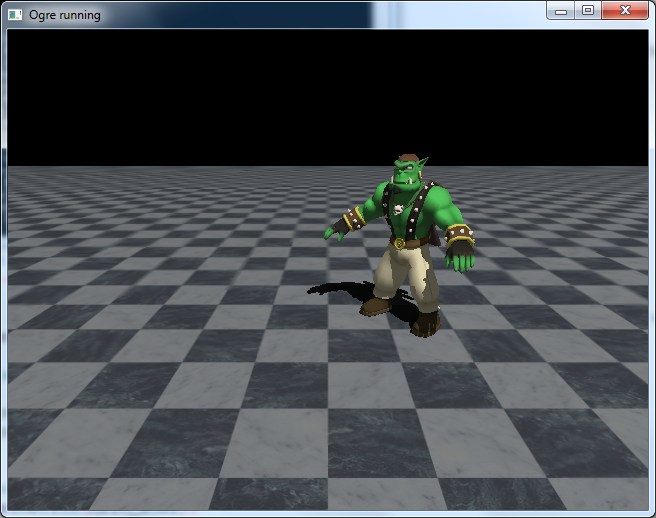
\includegraphics[width=0.7\textwidth]{meshanim.png}
\end{center}

The code you see in this project is actually a simplified version of an OGRE \texttt{Character} sample application. You can find the full version with all 13 animations, smooth transitions between animations and floating camera in the OGRE SDK\footnote{Check out the file \texttt{Samples/Character/include/SinbadCharacterController.h}}.

Complex meshes like the one we use here, their skeletons and animations can be created with modeling tools like Blender and then exported to OGRE format using exporters\footnote{\url{http://www.ogre3d.org/tikiwiki/tiki-index.php?page=Blender+Exporter}} provided by OGRE. The ``Sinbad'' character was created in Blender, so you can open \verb#data/Character/Sinbad.blend# and do with it whatever you want\footnote{The ``Sinbad'' model is licensed under CC-BY-SA by Zi Ye, i.e. you can use it freely given that you give appropriate credit. Check out the appropriate README file.}. To access the list of animations open ``Dope Sheet" in one of the panels, choose ``Action Editor"\footnote{\url{http://wiki.blender.org/index.php/Doc:2.6/Manual/Animation/Editors/DopeSheet/Action}} and then you will see a drop-down list with the available animations.

\begin{exercise}{7*}{2}
This bonus exercise offers you a variety of interesting things you can do. Implement all of them, any of them or any combination of them. Depending on the amount of effort you can get 1-2 bonus points.
\\
\\
\textbf{More animations}\\
Study the code in OGRE SDK \verb#Samples/Character# and add more animations to our application: idle animation, jump, smooth transitions, sword movements, etc. Add camera behaviour if you like. This exercise relies heavily on your coding skills, if you are friends with C++, this exercise should be mostly copy-pasting to correct places.
\\
\\
\textbf{Export from Blender}\\
Create a simple custom mesh with an armature and an animation in Blender (e.g. use the one you made in the previous practice session), export it to OGRE using the BlenderExporter\footnote{\url{http://www.ogre3d.org/tikiwiki/tiki-index.php?page=Blender+2.5+Exporter}} and use it in the application.
\ \\
\ \\
\textbf{Terrain}\\
In OGRE official Basic Tutorial 3: ``Terrain, Sky, and Fog"\footnote{\url{http://www.ogre3d.org/tikiwiki/tiki-index.php?page=Basic+Tutorial+3}} you can learn how to create terrains, sky (as we already did in Exercise 3) and fog resulting in a scene like this:
\begin{center}
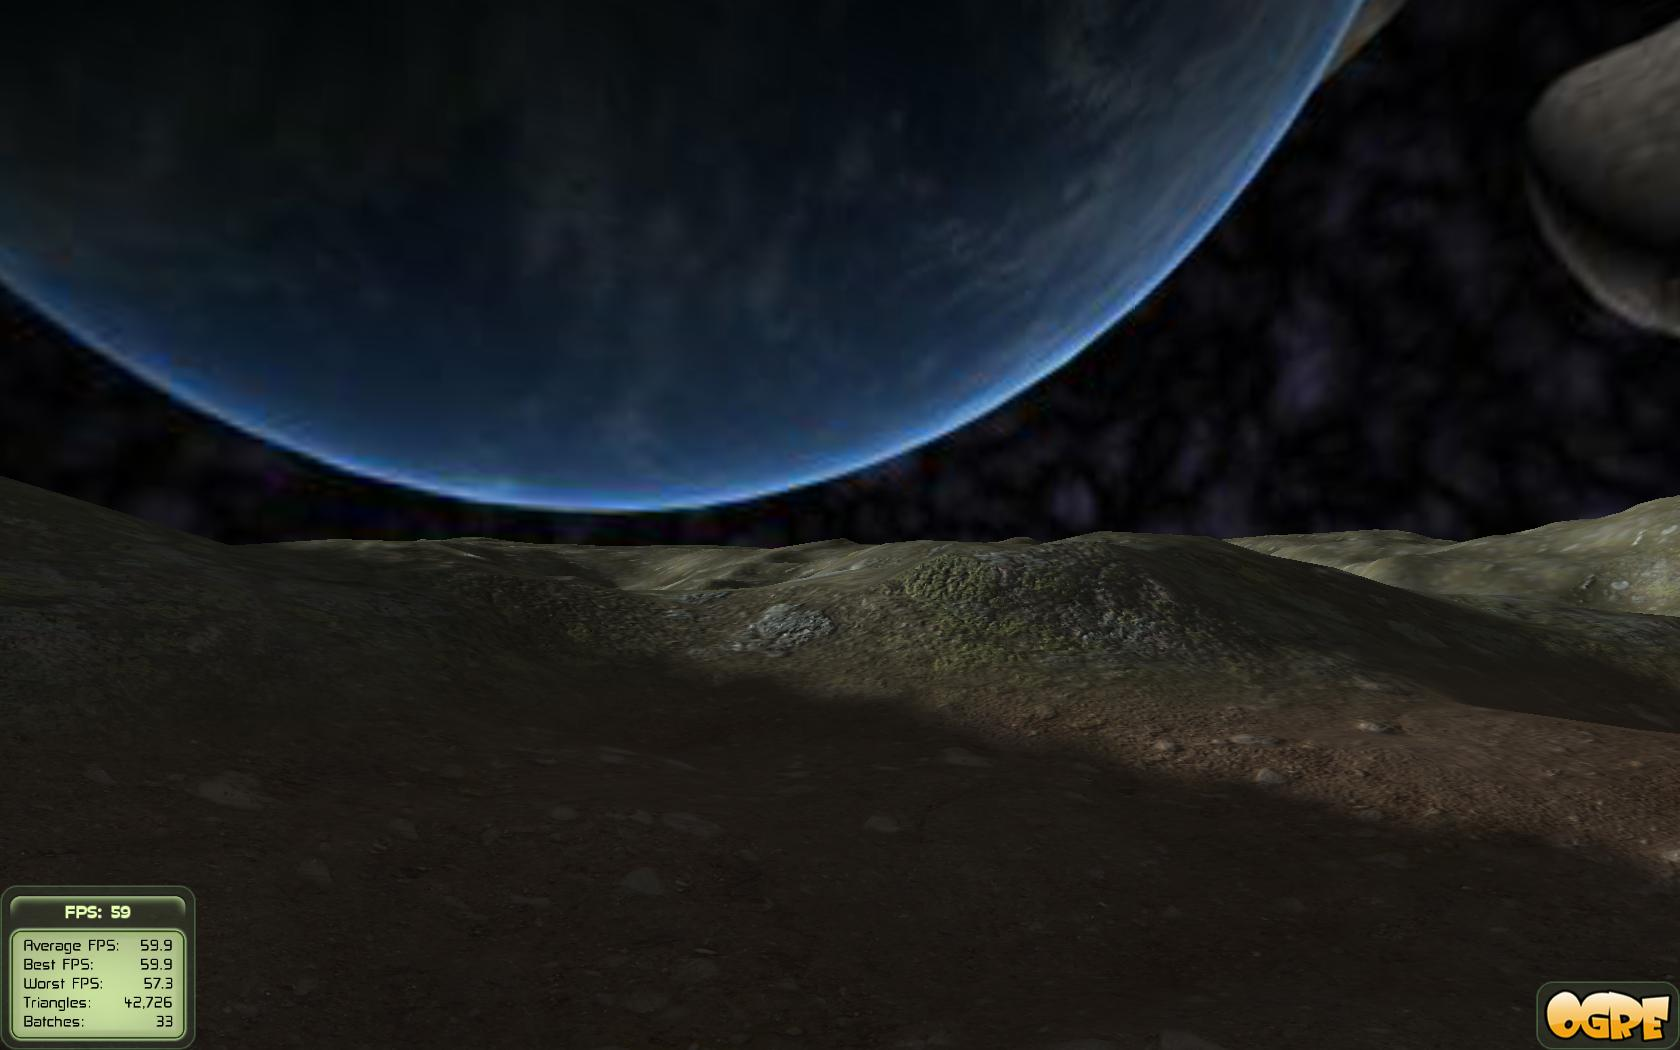
\includegraphics[width=0.7\textwidth]{terrain.jpg}
\end{center}
Take your animated character and place him into such a world. Choose details to your own liking: terrain, sky, light, shadows, textures, reflections, army of ogres, other creatures\footnote{Look inside \texttt{media/models} folder of OGRE SDK for more meshes and characters} and perhaps a mysterious reflective torus knot in the middle of everything...
\end{exercise}


\section{Particle systems}
Specialized functionality in OGRE is implemented via separate modules called ``plugins''. This way you are free to only use the parts of the library that you need in your project. Open project \verb#4_OgreParticles#. Have a look at the following line in the very beginning of the \verb#run()# function:
\begin{verbatim}
  mRoot = new Ogre::Root("plugins.cfg");
\end{verbatim}
It tells OGRE the name of a file in \verb#bin# directory (or whatever directory your app is launched from), listing which plugins must be loaded. Inside that file you will see that a plugin called ParticleFX is enabled. This plugin lets you add \emph{particle system} objects to your scene. A particle system is typically described using a \emph{particle script} in the resource files, which resembles \verb#.material# files we have seen before. Open \verb#data/Examples.particle# and study it.

\begin{exercise}{8}{0.5}
To complete this exercise do the following:
\begin{enumerate}
	\item Make particle source follow mouse movements. For that you will need to add mouse listener in the way analogous to the way how keyboard listener is added. See comments in the code.
	\item Play with different parameters of the particle system description. Modify the particle script so that the particles would fly out of the source in random directions, somewhat like fireworks or Bengal lights.
\end{enumerate}
\end{exercise}


\end{document}
